\section {The PCB}
\begin{figure}[h]
  \centering
  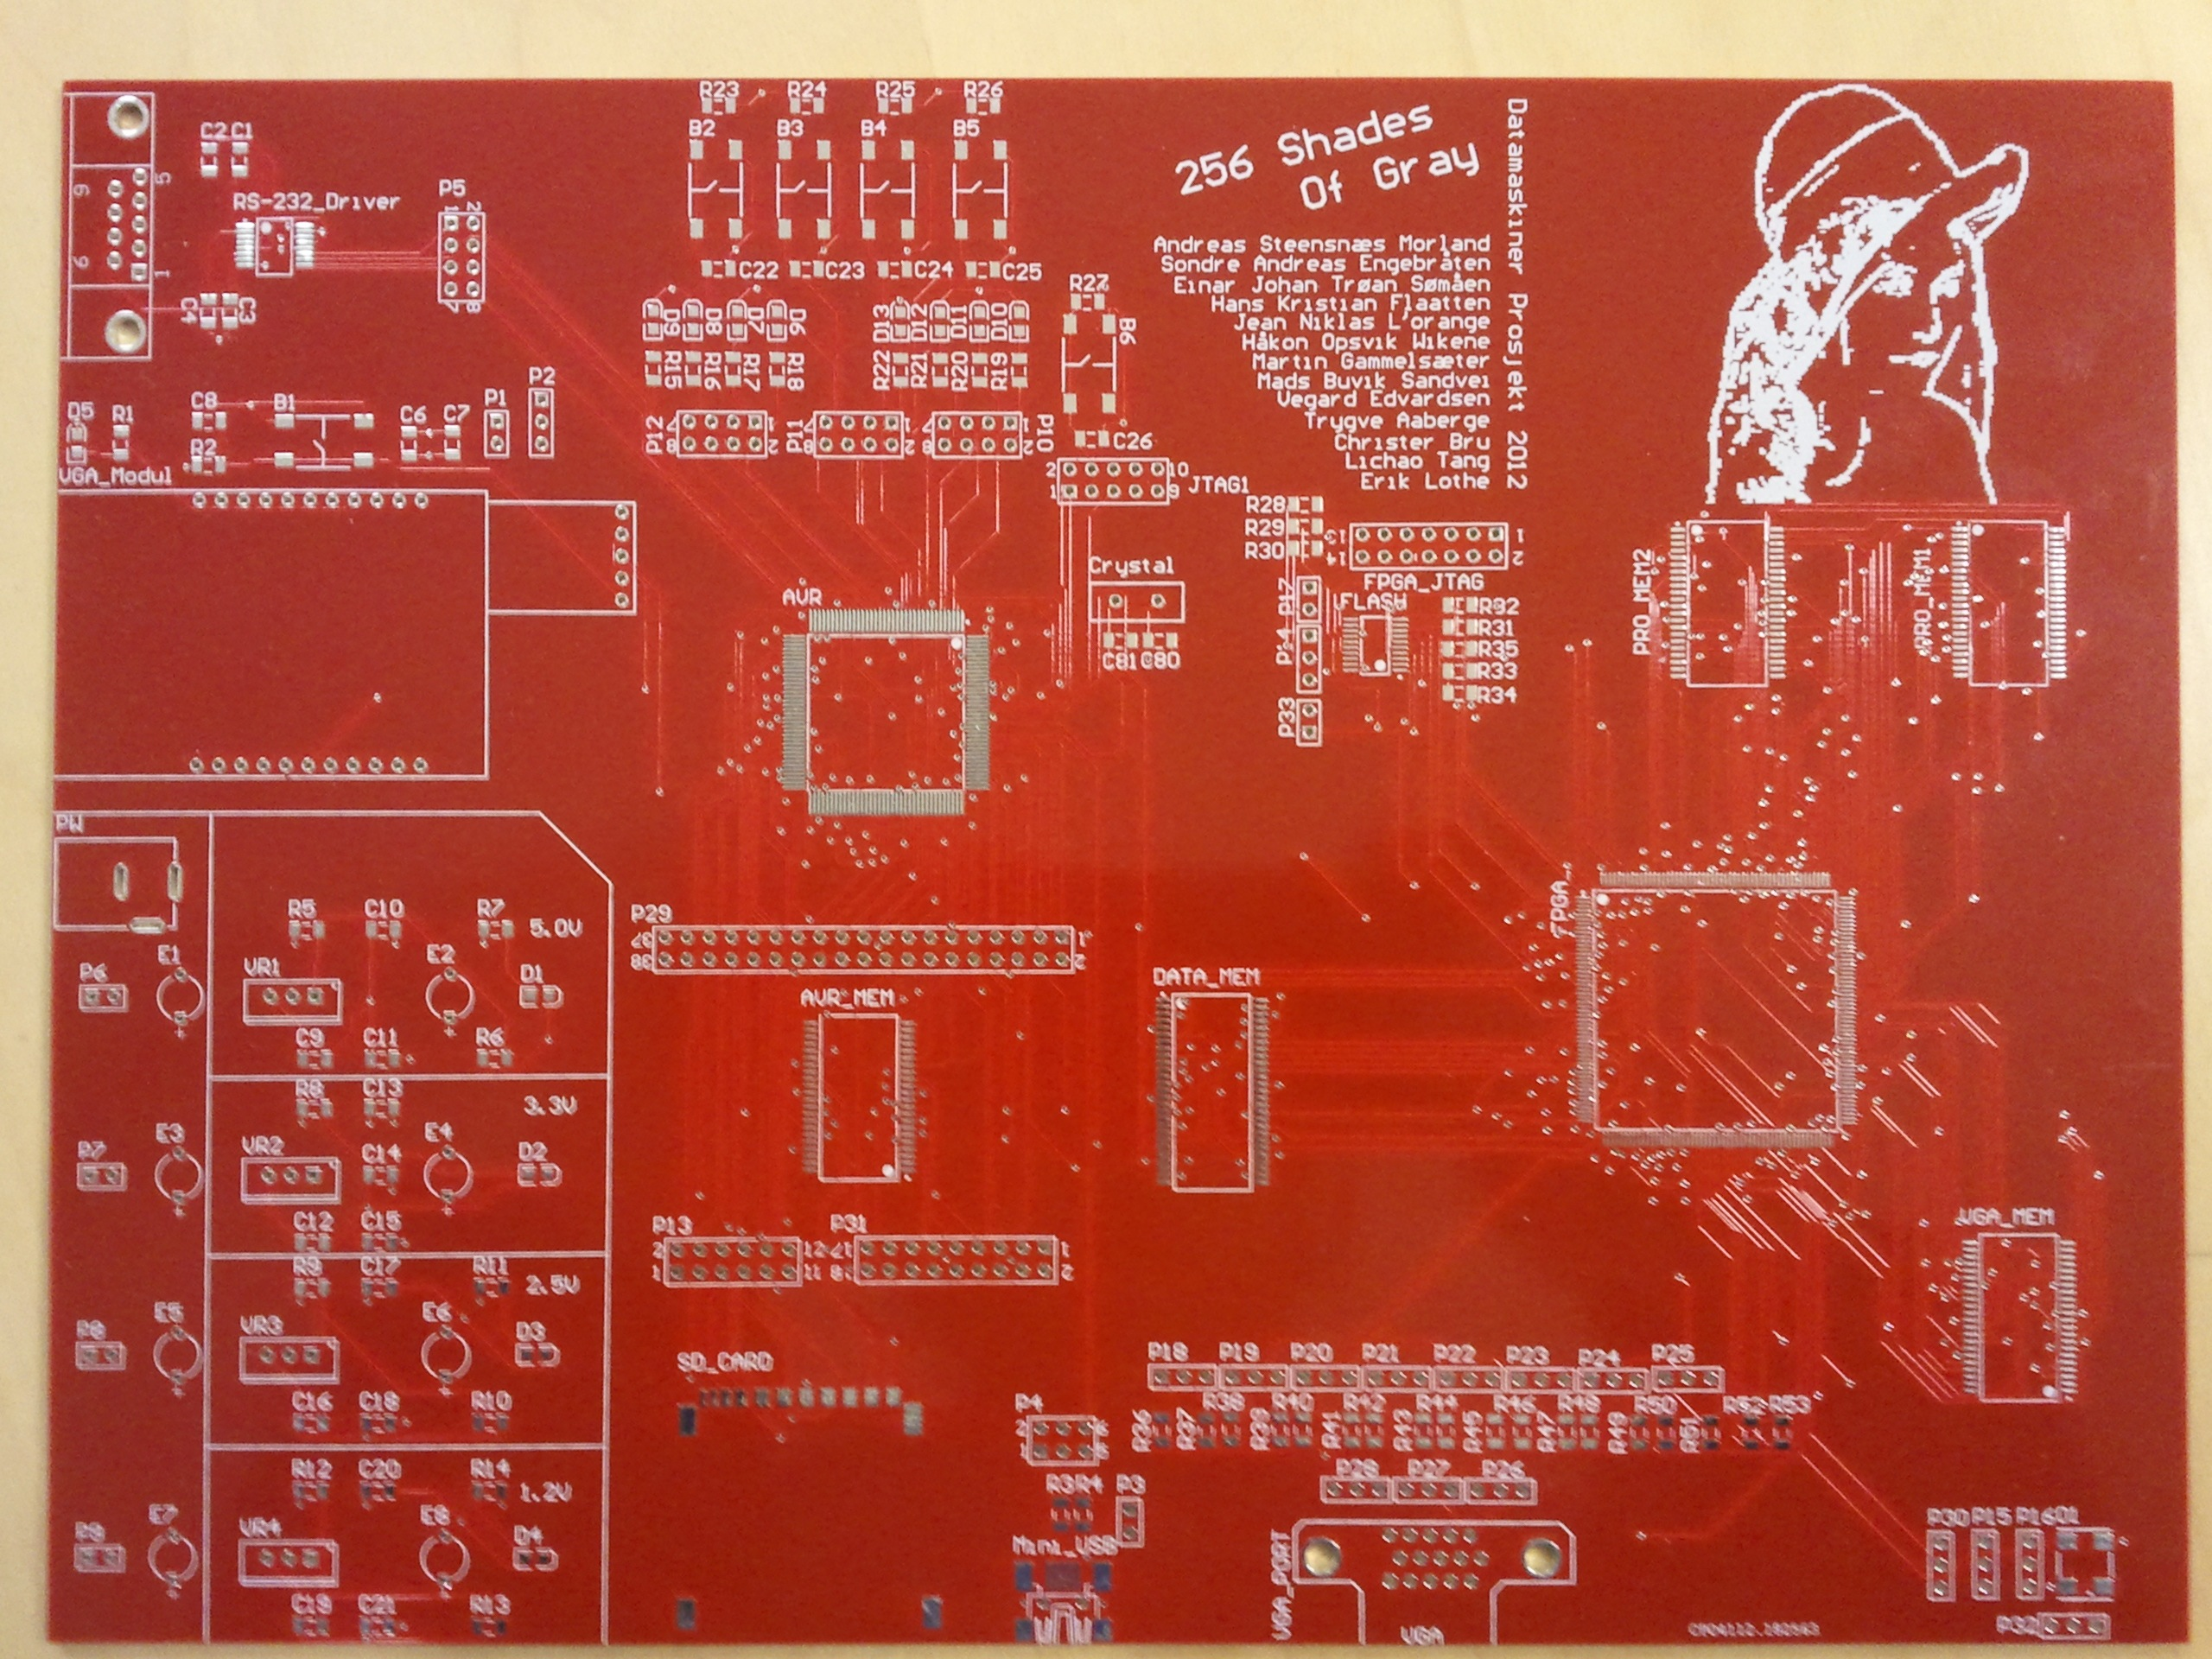
\includegraphics[width=0.8\textwidth]{fig/pcb/pcbwithoutcomp.jpg}
  \caption{The PCB without Components}
  \label{fig:pcb}
\end{figure}
When the PCB finally arrived from production we started soldering, this proved to be a bit
more difficult than originally anticipated. First, we tested whether there were short circuit in the board itself. We used multimeter to test that there was no current that goes from different layer. Then, we started to solder with the power supply, one power plane at time, testing the board for short circuit after each iteration. The table 5.1 shows the observerd voltage from each plane. 
\begin{table}[h]
  \centering
  \begin{tabularx}{\textwidth}{l l l l}\toprule
    \thx{Test} & \thx{Result} & \thx{Passed} 
    \\ 
	 \midrule
    Power supply 12.0V               &Measured 12.045  & OK  \\	
\midrule
    Power supply 5.0V               &Measured 4.995  & OK  \\
    \midrule
    Power supply 3.3V                   & Measured 3.286 & OK  \\
    \midrule
    Power supply 2.5V                 & Measured 2.510 & OK \\
    \midrule
    Power supply 1.2V            & Measured 1.240 & OK  \\
    
    \bottomrule
  \end{tabularx}
  \caption{Results of power supply}
  \label{fig:pcb}
\end{table}


Then we started with AVR, getting the AVR in place was particularly difficult, but after asked Tufte we lent a glue stick to put some glue on it to get more friction, thus keeping it in place while we soldered.

After about a days work we managed to completely destroy a pin on the AVR, therefore we had to start from scratch on a new board. On this new board we started with the AVR and FPGA, as they are the hardest components to solder. After each side on the AVR and FPGA, we tested for short circuits. As none were found, we moved on to the power supply, as well as JTAGs , FLASH and LEDs. In order to check the PCB was working, the AVR and FPGA groups tested the PCB board without the capacitors, after both groups tested that they could connect to the AVR and FPGA respectively, we began to solder the rest part of the PCB. 
\begin{figure}[h]
  \centering
  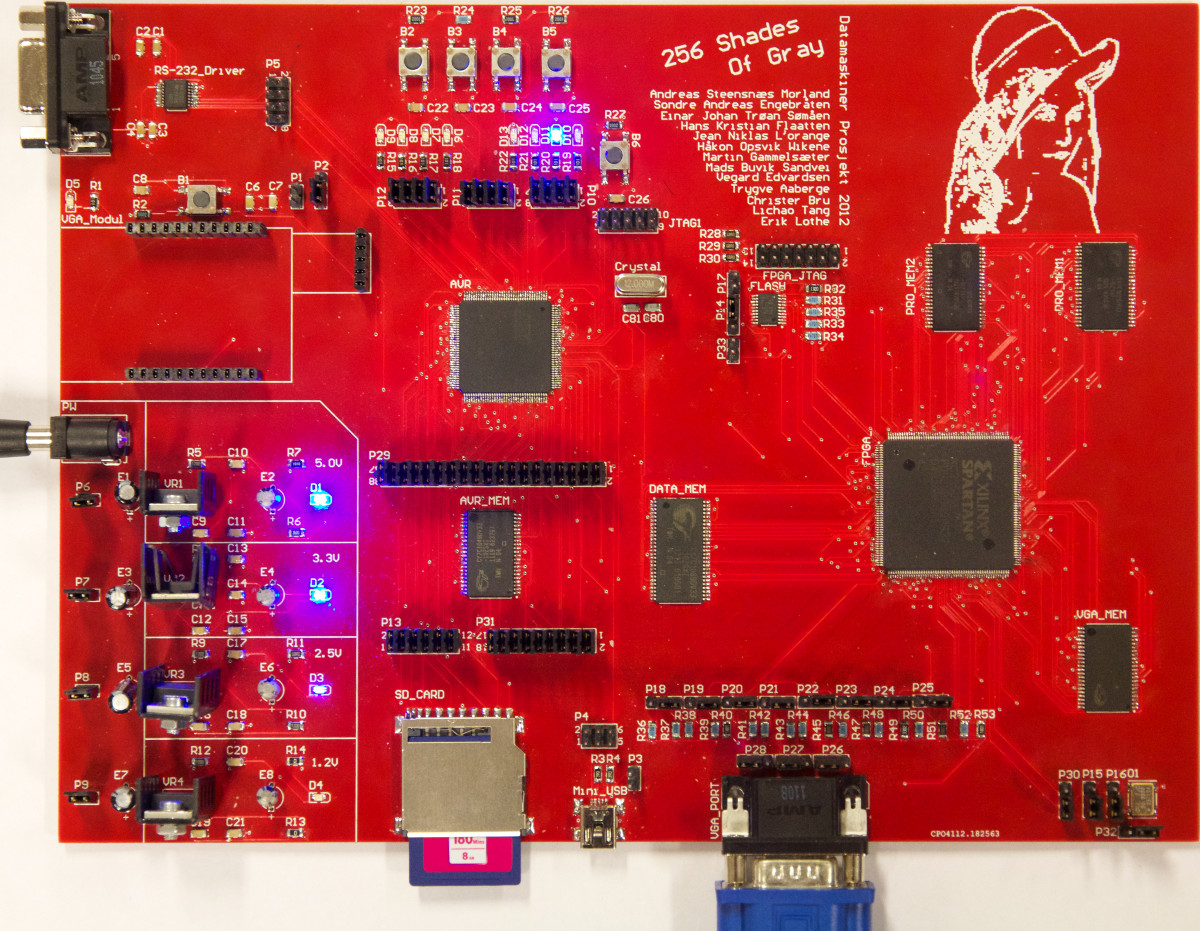
\includegraphics[width=0.8\textwidth]{fig/pcb/pcbwithcomp.jpg}
  \caption{The PCB With All The Components}
  \label{fig:pcb}
\end{figure}
